\documentclass[11pt,a4paper]{article}

\usepackage{amsmath}
\usepackage{amssymb}
\usepackage{algorithm}
\usepackage{algorithmic}
\usepackage{graphicx}
\usepackage{geometry}
\geometry{margin=2.5cm}

\usepackage{tikz}
\usetikzlibrary{arrows.meta, positioning}


\title{Learning a Data-Driven Beam Search Heuristic Using a Feed-Forward Neural Network and Genetic Algorithms}
\author{}
\date{}

\begin{document}
\maketitle

\section{Overview}

This work proposes a learning framework for constructing a data-driven heuristic to guide Beam Search in combinatorial optimization problems. A feed-forward neural network (FFNN) is used to parameterize the heuristic function. Instead of relying on gradient-based training, the network weights are optimized using a Genetic Algorithm (GA).

Each individual in the GA population represents a complete set of neural network weights. The quality of an individual is evaluated by embedding the neural network inside Beam Search and measuring the average solution quality obtained on a set of training instances. Validation instances are used exclusively to monitor generalization.

Formally, the learning problem is defined as:
\[
\max_{\theta} \; \frac{1}{|T|} \sum_{I \in T} f(\text{BeamSearch}(I, h_\theta)),
\]
where $T$ denotes the training set, $h_\theta$ is the neural heuristic parameterized by weights $\theta$, and $f(\cdot)$ measures solution quality.

\section{Neural Network Model}

The heuristic is represented by a multilayer perceptron with an arbitrary number of hidden layers and user-defined units per layer. Supported activation functions include hyperbolic tangent, ReLU, and sigmoid.

For each layer $l$, forward propagation is defined as:
\[
\mathbf{z}^{(l+1)} = W^{(l)} \mathbf{a}^{(l)} + b^{(l)}, \quad
\mathbf{a}^{(l+1)} = \phi(\mathbf{z}^{(l+1)}),
\]
where $W^{(l)}$ and $b^{(l)}$ are the weight matrix and bias vector, respectively, and $\phi$ denotes the activation function.

All weights and biases are flattened into a single vector, which forms the chromosome of a GA individual.

\section{Fitness Evaluation}

Given a candidate weight vector:
\begin{enumerate}
    \item The weights are loaded into the FFNN.
    \item Beam Search is executed on each training instance using the neural heuristic.
    \item The size of the best sequence obtained for each instance is recorded.
\end{enumerate}

The fitness value is computed as the average solution quality over all training instances. Validation performance is computed analogously on a separate dataset and is used only for reporting.

\section{Genetic Algorithm}

The optimization process follows a population-based evolutionary scheme.

\subsection{Initialization}

Each individual is initialized by sampling weights uniformly from a predefined interval [$-w, w$].

\subsection{Elitism}

A fixed number of top-performing individuals are copied unchanged into the next generation.

\subsection{Mutation}

Several individuals are generated completely at random (random immigrants). This mechanism promotes exploration and maintains population diversity.

\subsection{Offspring Generation}

Three alternative parent-selection strategies are supported:

\begin{itemize}
    \item \textbf{RKGA}: Two parents are selected uniformly at random, and each gene is inherited from either parent with probability $0.5$.
    \item \textbf{BRKGA}: One parent is selected from the elite set and one from the non-elite set. Each gene is inherited from the elite parent with a predefined probability.
    \item \textbf{Lexicase Selection}: Training instances are randomly shuffled. Individuals are filtered iteratively by retaining those achieving the best performance on each instance. Parents are selected randomly from the remaining candidates.
\end{itemize}

\subsection{Replacement and Termination}

The new population consists of elites, mutants, and offspring. The algorithm terminates once a predefined time limit is reached. The best individual encountered during training is continuously tracked and stored.

\section{Overall Learning Procedure}

The learning process alternates between evolutionary optimization of network weights and evaluation through (iterative multi-source) Beam Search. Importantly, the neural network does not directly predict solutions; instead, it learns how to guide the search procedure. This places the method within the class of neuro-evolutionary hyper-heuristics.

\section{Algorithm}

\begin{algorithm}[H]
\caption{GA-Based Learning of a Beam Search Heuristic}
\begin{algorithmic}[1]
\STATE Initialize population $P$ with random neural network weights
\STATE Evaluate all individuals on training set $T$
\STATE Store best solution $\theta^\ast$
\STATE $start \leftarrow$ current time
\WHILE{current time $- start < T_{\max}$}
    \STATE Sort $P$ by fitness (descending)
    \STATE Initialize empty population $P'$
    \STATE Copy top $n_{elites}$ individuals from $P$ to $P'$
    \FOR{$i = 1$ to $n_{mutants}$}
        \STATE Create random individual $x$
        \STATE Evaluate $x$ on $T$
        \STATE Add $x$ to $P'$
        \STATE Update $\theta^\ast$ if improved
    \ENDFOR
    \FOR{$i = 1$ to $n_{offspring}$}
        \STATE Select parents using RKGA, BRKGA, or Lexicase
        \STATE Generate offspring by crossover
        \STATE Evaluate offspring on $T$
        \STATE Add offspring to $P'$
        \STATE Update $\theta^\ast$ if improved
    \ENDFOR
    \STATE $P \leftarrow P'$
\ENDWHILE
\STATE \textbf{return} best weights $\theta^\ast$
\end{algorithmic}
\end{algorithm}


\begin{figure}[t]
	\centering
	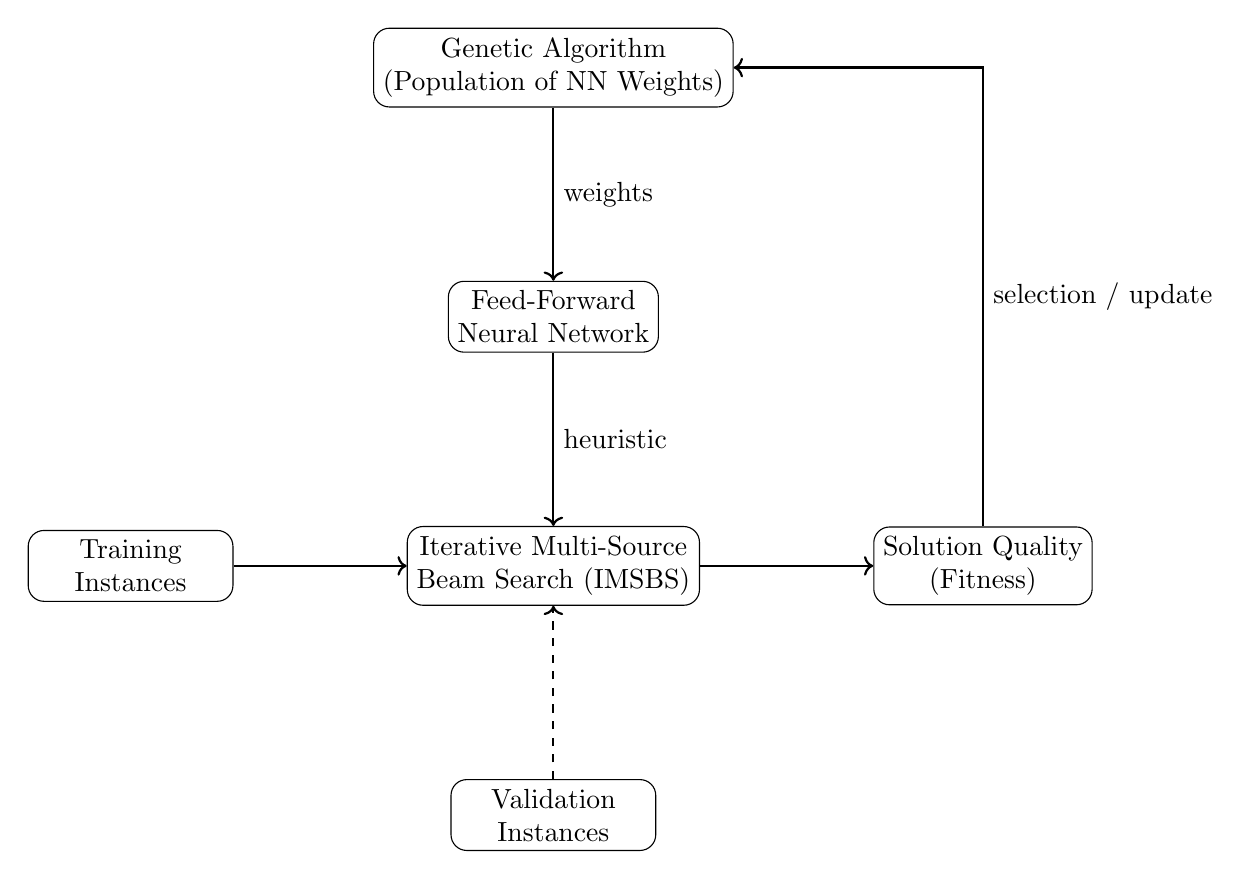
\begin{tikzpicture}[
		box/.style={draw, rounded corners=2mm, align=center, minimum width=3.2cm, minimum height=1cm},
		smallbox/.style={draw, rounded corners=2mm, align=center, minimum width=2.6cm, minimum height=0.9cm},
		arrow/.style={->, thick},
		node distance=2.2cm
		]
		
		% GA block
		\node[box] (ga) {Genetic Algorithm\\(Population of NN Weights)};
		
		% NN
		\node[smallbox, below=of ga] (nn) {Feed-Forward\\Neural Network};
		
		% Beam Search
		\node[box, below=of nn] (bs) {Iterative Multi-Source\\Beam Search (IMSBS)};
		
		% Training instances
		\node[smallbox, left=of bs] (train) {Training\\Instances};
		
		% Solutions / fitness
		\node[smallbox, right=of bs] (fitness) {Solution Quality\\(Fitness)};
		
		% Arrows
		\draw[arrow] (ga) -- node[right]{weights} (nn);
		\draw[arrow] (nn) -- node[right]{heuristic} (bs);
		\draw[arrow] (train) -- (bs);
		\draw[arrow] (bs) -- (fitness);
		\draw[arrow] (fitness.north) |- node[pos=0.25,right]{selection / update} (ga.east);
		
		% Validation (optional)
		\node[smallbox, below=of bs] (val) {Validation\\Instances};
		\draw[arrow,dashed] (val) -- (bs);
		
	\end{tikzpicture}
	
	\caption{Learning framework integrating a Genetic Algorithm with Iterative Multi-Source Beam Search (IMSBS).
		The GA evolves neural network weights. For each individual, the FFNN provides a heuristic used by IMSBS on training
		instances. The resulting solution quality defines fitness, which drives evolutionary selection. Validation
		instances are used only for monitoring generalization.}
	\label{fig:ga_imsbs}
\end{figure}


\section{Discussion}

The proposed framework learns heuristics rather than explicit solutions. The neural network is optimized exclusively through downstream search performance, enabling learning in non-differentiable settings. This tightly coupled integration of evolutionary learning and Beam Search allows the system to adapt its guidance strategy to the structure of the problem instances.

\end{document}

